% lecture11.tex — Transversality

\section{Transversality}

Earlier, we saw that transversality is stable under small perturbations. Today, we'll use Sard's theorem to show that transversal maps are \emph{generic} in the sense that any smooth map can be deformed by an arbitrarily small amount into a transversal map.

(Think as a smooth family of maps $f_s \colon M \to N$, $s \in S$.)

\begin{theorem}{Transversality Theorem}{transversality-thm}
    Suppose $F \colon M \times S \to N$ is a smooth map of manifolds, where only $M$ has $\partial$, and let $P \subset N$ be a submanifold. If both $F$ and $F|_{\partial M \times S}$ are transversal to $P$, then for almost every $s \in S$, both $f_s$ and $f_s|_{\partial M}$ are transversal to $P$.
\end{theorem}

\begin{proof}
    The preimage $Q = F^{-1}(P) \subset M \times S$ is a submanifold with boundary $\partial Q = Q \cap (\partial M \times S)$. Let $\pi \colon Q \to S$ be the projection.

    We'll show that \textcircled{1} $f_s \pitchfork P$ whenever $s$ is a regular value for $\pi$, and \textcircled{2} $f_s|_{\partial M} \pitchfork P$ whenever $s$ is a regular value for $\pi|_{\partial Q}$. The theorem will then follow from Sard.

    Note that the second claim is a special instance of the first claim, for the map $F|_{\partial M \times S} \colon \partial M \times S \to N$ of boundaryless manifolds, so it suffices to show \textcircled{1}.

    In order to show $f_s \pitchfork P$, we need to show that, for any $x \in M$ with $f_s(x) = y \in P$, the composition $T_x M \xrightarrow{d(f_s)_x} T_y N \xrightarrow{p} T_y N / T_y P$ is surjective. (Here $d(f_s)_x(v) = dF_{(x,s)}(v, 0)$.)

    Since $F \pitchfork P$, we know that
    \[
        T_{(x,s)}(M \times S) = T_x M \times T_s S \xrightarrow{dF_{(x,s)}} T_y N \xrightarrow{p} T_y N / T_y P
    \]
    is surjective. Moreover, by the regularity assumption, $d\pi_{(x,s)} \colon T_{(x,s)} Q \to T_s S$ is surjective.

    Since $T_{(x,s)} Q \subset T_x M \times T_s S$ is in the kernel of $p \circ dF_{(x,s)}$, it follows that the restriction $p \circ dF_{(x,s)}|_{T_x M \times 0} = p \circ d(f_s)_x$ is surjective, as desired.
\end{proof}

\begin{corollary}{Transversal Maps are Generic (Euclidean Target)}{transversal-generic-euclidean}
    Transversal maps are generic when the target manifold $N$ is $\R^\ell$.
\end{corollary}

\begin{proof}
    If $f \colon M \to \R^\ell$ is any smooth map, take $S$ to be an open ball of $\R^\ell$, and define $F \colon M \times S \to \R^\ell$, $(x, s) \mapsto f(x) + s$.

    For any fixed $x$, this is obviously a submersion, so transversal to any submanifold $P \subset \R^\ell$.

    Thanks to the transversality theorem, $f_s(x) = f(x) + s$ is transversal to $P$, for almost every $s \in S$, where $s$ may be taken to be arbitrarily small.
\end{proof}

For an arbitrary target manifold $N \subset \R^\ell$, the proof of genericity of transversal maps is essentially the same; we just need to project the shifted map down to $N$.

\begin{lemma}{$\varepsilon$-Neighborhood Theorem}{epsilon-neighborhood}
    For any manifold $N \subset \R^\ell$, there is a smooth positive function $\varepsilon \colon N \to \R_{>0}$ such that each point $w \in N^\varepsilon := \{w \in \R^\ell \mid \|w - y\| < \varepsilon(y) \text{ for some } y \in N\}$ has a unique closest point $\pi(w)$ in $N$. Moreover, the map $\pi \colon N^\varepsilon \to N$ is a submersion.

    (See pp.~71--72 of Guillemin--Pollack for the proof.)
\end{lemma}

\begin{center}
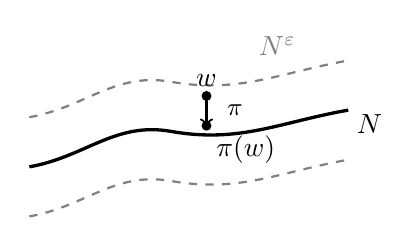
\begin{tikzpicture}[scale=0.9]
    % Manifold N (curve)
    \draw[very thick] (-2,-0.5) to[out=10,in=170] (0,0) to[out=-10,in=190] (2.5,0.3);
    \node at (2.8,0.1) {$N$};
    % Epsilon neighborhood (tube)
    \draw[thick,dashed,gray] (-2,-0.5+0.7) to[out=10,in=170] (0,0.7) to[out=-10,in=190] (2.5,1);
    \draw[thick,dashed,gray] (-2,-0.5-0.7) to[out=10,in=170] (0,-0.7) to[out=-10,in=190] (2.5,-0.4);
    \node[gray] at (1.5,1.2) {$N^\varepsilon$};
    % Point w and projection
    \fill (0.5,0.5) circle (2pt) node[above] {$w$};
    \draw[->,thick] (0.5,0.5) -- (0.5,0.08);
    \fill (0.5,0.08) circle (2pt) node[below right] {$\pi(w)$};
    \node at (0.9,0.3) {\small $\pi$};
\end{tikzpicture}
\end{center}

\begin{corollary}{Submersive Family}{submersive-family}
    Let $f \colon M \to N$ be a smooth map, where only $M$ has boundary. Then there is an open ball $S$ in some Euclidean space and a smooth map $F \colon M \times S \to N$ such that $F(x, 0) = f(x)$, and for any fixed $x \in M$, the map $S \to N$, $s \mapsto F(x, s)$, is a submersion. In particular, both $F$ and $F|_{\partial M \times S}$ are submersions.
\end{corollary}

\begin{proof}
    Let $S$ be the unit open ball in $\R^\ell \supset N$, and define
    \[
        F(x, s) = \pi\bigl(f(x) + \varepsilon(f(x)) s\bigr).
    \]
    Since $\pi \colon N^\varepsilon \to N$ restricts to the identity on $N$, $F(x, 0) = f(x)$. Since $s \mapsto f(x) + \varepsilon(f(x)) s$ and $\pi$ are compositions of two submersions, it is a submersion.
\end{proof}

\subsection{Transversality Homotopy and Extension Theorems}

\begin{theorem}{Transversality Homotopy Theorem}{transversality-homotopy}
    For any smooth map $f \colon M \to N$ and a submanifold $P \subset N$, where only $M$ has $\partial$, there exists a smooth map $g \colon M \to N$ homotopic to $f$ such that $g \pitchfork P$ and $g|_{\partial M} \pitchfork P$.
\end{theorem}

\begin{proof}
    For the family of maps $F$ in the corollary, the transversality theorem implies that $f_s \pitchfork P$ and $f_s|_{\partial M} \pitchfork P$ for almost all $s \in S$, but each $f_s$ is homotopic to $f$, with homotopy $M \times I \to N$, $(x, t) \mapsto F(x, ts)$.
\end{proof}

We'll actually need a slightly stronger form of this theorem:

\begin{theorem}{Extension Theorem (Relative Transversality Homotopy)}{extension-thm}
    In the setting as above, where $P$ is a closed submanifold, suppose $C \subset M$ is a closed subset such that $f \pitchfork P$ on $C$ and $f|_{\partial M} \pitchfork P$ on $C \cap \partial M$.

    Then there exists a smooth map $g \colon M \to N$ homotopic to $f$ such that $g \pitchfork P$, $g|_{\partial M} \pitchfork P$, and $g = f$ on a neighborhood of $C$.

    (See pp.~72--73 of Guillemin--Pollack for the proof. The idea is to modify $F \colon M \times S \to N$ where $\tau \colon M \to [0,1]$ is a smooth bump function that is $0$ on $C$ and $1$ outside of an open neighborhood, by setting $G \colon M \times S \to N$, $(x, s) \mapsto F(x, \tau(x) s)$.)
\end{theorem}

\begin{corollary}{Extension of Transversality}{extension-transversality}
    If $f \colon M \to N$ is a smooth map such that $f|_{\partial M} \colon \partial M \to N$ is transversal to $P \subset N$, then there exists a map $g \colon M \to N$ homotopic to $f$ rel $\partial$ (i.e.\ $g|_{\partial M} = f|_{\partial M}$) such that $g \pitchfork P$.
\end{corollary}
